\section{OpenWorkflow: FSM Workflow Authoring Tools}
\label{sec: app-dev-fsm}

In addition to creating DNN-based object detectors, developers need to write
custom logic to implement the WCA task model running on the cloudlet. In this
section, we introduce OpenWorkflow, an FSM authoring tool that provides a Python
library and a GUI to enable fast implementation to allow for quick development
iteration.

As discussed in Section~\ref{sec: app-dev-fsm-representation}, the WCA cloudlet
logic can be represented as a finite state machine. The FSM representation
allows us to impose structure and provide tools for task model implementation.
OpenWorkflow consists of a web GUI that allows users to visualize and
edit a WCA FSM within a browser, a python library that supports the creation and
execution of a FSM, and a binary file format that efficiently stores the FSM.
The OpenWorkflow video demo can be found at \url{https://youtu.be/L9ugONLpnwc}.

\subsection{OpenWorkflow Web GUI}

\begin{figure}
    \centering
    \fbox{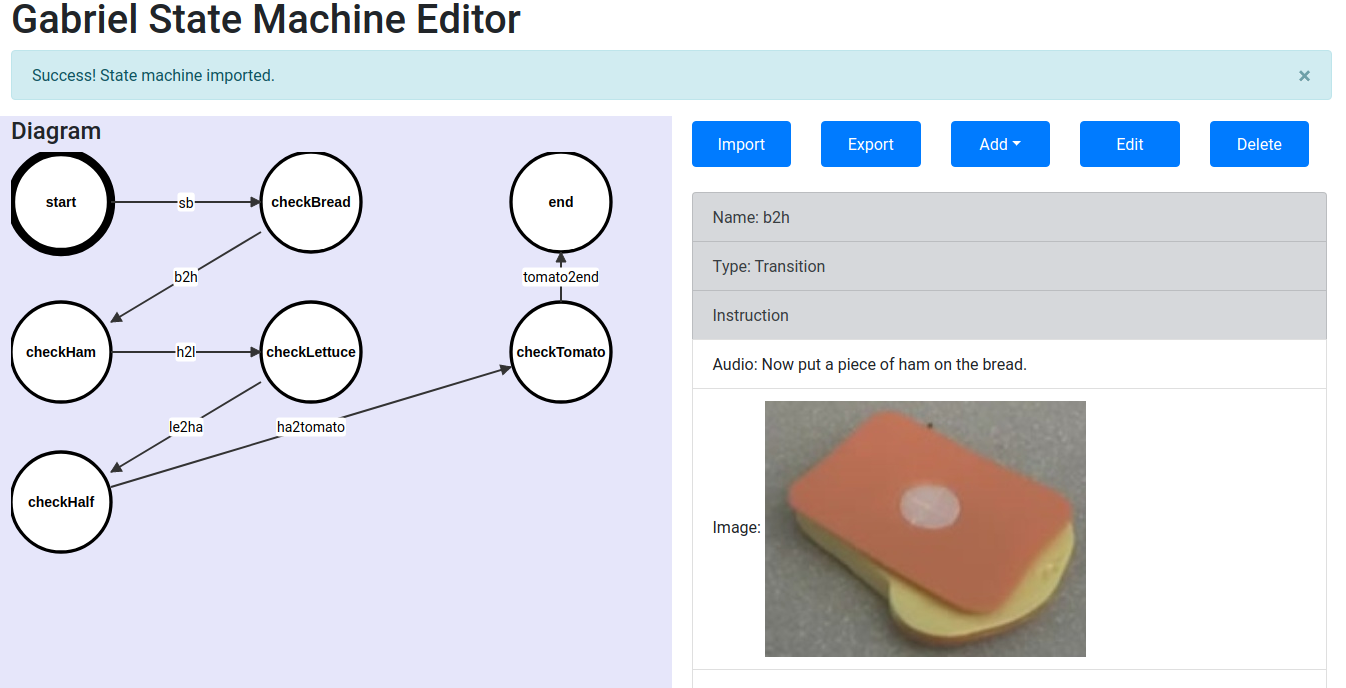
\includegraphics[trim={0 0 0 0},width=\linewidth]{FIGS/fsm-web-gui}}
	\caption{OpenWorkflow Web GUI}
    \label{figs:fsm-web-gui}
\end{figure}

Figure~\ref{figs:fsm-web-gui} shows the OpenWorkflow web GUI. Users can create a WCA
FSM from the GUI by editing states and transitions. State processors, e.g. the
computer vision processing logic to run in a given state, can be specified by a
container url. User guidance can be added through adding text, video urls or by
uploading images. The Web GUI also supports import and export functionalities to
interface with other WCA tools. The exported FSM is in a custom binary format
and can be executed by the OpenWorkflow Python library.

The GUI is implemented as a pure browser-based user interface, using
React~\cite{staff2016react}. No web backend is needed. This makes the GUI easy
to set up and deploy. The user only needs to open an HTML file in a browser to 
use the tool.

\subsection{OpenWorkflow Python Library}

Another way to programmatically create a FSM is through the OpenWorkflow Python
library. The library provides python APIs to create and modify FSMs. The python
APIs provides additional interfaces to add custom computer vision processing as
functions and ad hoc transition predicates for customization. 

In addition, the Python library provides a state machine executor that takes a
WCA FSM (e.g. made with the Web GUI) and launches a WCA program using the
Gabriel platform. The program is then ready to be connected by Gabriel Android
Client. The WCA program follows the logic defined in the state machine. A
Jupyter Notebook~\cite{kluyver2016jupyter} is also provided to make it possible to launch the program from
a browser. This library has been made available on The Python Package Index for
easy installation.

\subsection{OpenWorkflow Binary Format}

We define a custom FSM binary format for WCAs that can be read and wrote using
multiple programming languages. We use the serialization library Protocol
Buffers to generate language-specific stub code.
Figure~\ref{figs:fsm-binary-format} shows a summary of the serialization format.


\begin{figure}
\small
\begin{lstlisting}
// represents the trigger condition
message TransitionPredicate {
  string name = 1;
  string callable_name = 2; 
  map<string, bytes> callable_kwargs = 3; // arguments
  string callable_args = 4; // arguments
}

message Instruction {
  string name = 1;
  string audio = 2; // audio in text format.
  bytes image = 3;
  bytes video = 4;
}

message Transition {
  string name = 1;
  // function name of the trigger condition
  repeated TransitionPredicate predicates = 2;
  Instruction instruction = 3;
  string next_state = 4;
}

// represent feature extraction modules
message Processor {
  // input are images
  // outputs are key/value pairs that represents application state
  string name = 1;
  string callable_name = 2; 
  map<string, bytes> callable_kwargs = 3; // arguments
  string callable_args = 4; // arguments
}

message State {
  string name = 1;
  repeated Processor processors = 2; // extract features
  repeated Transition transitions = 3;
}

message StateMachine {
  string name = 1;
  repeated State states = 2; // all states
  map<string, bytes> assets = 3; // shared assets
  string start_state = 4;
}
\end{lstlisting}
\caption{OpenWorkflow FSM Binary Format}
\label{figs:fsm-binary-format}
\end{figure}

% We observed that the
% implementation of a cognitive assistant mainly consists of components to
% identify user states using computer vision models, specify instructions to users
% based on the current state, and keep track of progress on the task. We created a
% a workflow modeling tool, SME, which can transform the process of completing a
% task into a specific model, substantially reducing the expert modeling effort
% required. By using a framework to reason about step-by-step application, along
% with workflow information from WE and object recognition models from OpenTPOD, SME
% also automatically generates a Gabriel executable application based on the
% modeled workflow.

% The applications SME generates are defined by a set of steps. Each state
% corresponds to the subset of steps that a user has completed. We use a FSM to
% keep track of the current state of a task and the future states that we should
% transition to when a user takes a certain action. Transitions among states are
% triggered by visual changes resulting from user actions. For example, the user
% might put a piece of ham on top of a piece of bread. In addition, each state has
% its own processing functions, which convert the current visual state into
% information that the application can understand. We provide a list of
% pre-defined processing functions, such as object detection DNNs. Task experts
% also have the flexibility to add custom processing functions when needed.
% Figure~\ref{fig:sme} shows a sample workflow as a finite state machine. Once the
% task expert finalizes a FSM, SME automatically compile the FSM to generate an
% executable application.